% Generated from saved CPU summaries by make_laptop.py.
\subsection{Repeated laptop CPU measurement with real attacked inputs}
\label{app:seg-laptop}
After the earlier rejected timing campaigns, a source audit identified a carryover imbalance: duplicate A/A labels had equal absolute positions but unequal preceding clean/attacked workload distributions. The caller also retained the previous output during the next invocation. A new prospective protocol balanced labels jointly by preceding workload and pair position, used the same callable for both labels, and released output after both clocks stopped. These changes form a bundle; the observations do not isolate an allocator, cache or scheduler mechanism. All earlier failures remain rejected.
Two prospectively tagged sessions reuse the same 20 frozen whole-image PGD pairs ($L_\infty=16/255$, 100 steps) and YOLOv8n-seg, with FP32 unfused inference, $640\times640$ native masks, confidence 0.25, IoU 0.45 and a fixed torchvision NMS backend. The i5-1335U laptop worker is pinned to logical CPU 2, one hardware thread of a P-core, with one intra-op and one inter-op thread. AboveNormal priority and HighQoS are process-local; the assistant application tree temporarily avoids CPU 2 and its SMT sibling 3, with journaled restoration. No power-plan or thermal-protection changes are made.
Each image/arm has 48 trials per A/A label; the primary median pools all 96 calls. All trials and spikes are retained. The endpoint spans prepared tensor to native-mask return, excluding output cleanup, decoding, transport, serialization and queueing. Each session independently requires at most two of 22 forward-reference medians outside $\pm3\%$ of baseline, both A/A MDEs at most 1\%, valid load pinning and environment/readback/restoration checks. Intervals below resample the 20 images 20,000 times, RNG seed 20261107; repeats are not independent images.
\begin{table*}[t]\centering
\caption{Two separately gated sessions on the same 20 frozen image pairs. Ratios are geometric means of per-image attack/clean median total latency. Both sessions pass; they are not independent image or device replications.}
\label{tab:seg-laptop}
\begin{tabular}{lrrrr}\toprule
Session & Total ratio [95\% CI] & Clean A/A MDE (\%) & Attacked A/A MDE (\%) & Drift flags\\\midrule
1 & 4.235134 [4.024954, 4.441712] & 0.996622 & 0.213432 & 1/22 \\
2 & 4.222968 [4.007657, 4.433076] & 0.829358 & 0.168182 & 0/22 \\
\bottomrule\end{tabular}\end{table*}
\begin{figure*}[t]\centering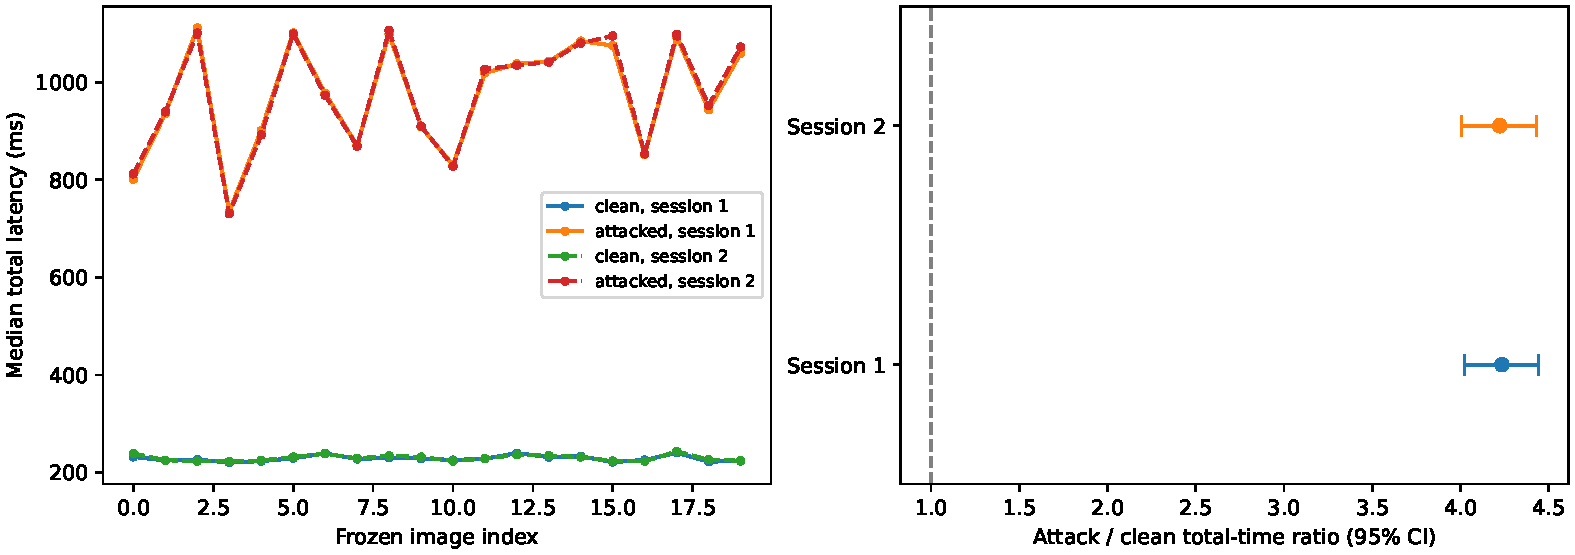
\includegraphics[width=.9\textwidth]{segmentation_extension/laptop_sessions.pdf}\caption{Saved per-image median latency and separate session ratio intervals. The same images and deterministic schedule are shared; no pooled cross-session interval is constructed.}\label{fig:seg-laptop}\end{figure*}
The first session clean MDE is close to the 1\% gate; the unrounded value was used for eligibility. Passing this median-based gate does not establish stable tail latency. Session 1 retains 24/1920 clean and 42/1920 attacked calls exceeding 1.5 times their image-specific median; session 2 retains 14/1920 and 52/1920. Each of these spikes has process-CPU/wall below 0.75. Their cause is unresolved. Process CPU time is coarsely quantized on this Windows installation; PDH nominal frequency is not treated as measured instantaneous clock.
The second session was registered after inspecting the first and reused its configuration without searching additional repeats or cores. Similar estimates are descriptive repeatability evidence, not an equivalence test. Neither session isolates NMS from mask work because isolated-stage profiling was omitted from this corrected total-only schedule. The installed native renderer chunks floating-point interpolation and returns uint8 masks; a monolithic full-float mask allocation is not assumed. Legacy shared hardware-helper line-ending differences between Git and executed working bytes are disclosed in the audit receipt; the prospective lock binds the exact executed SHA.
This result supports increased prepared-tensor computation cost in two sessions on one laptop and one model. It does not establish service denial, deadline misses, camera robustness, universal/localized patch effectiveness, ARM/Pi behavior, or timing validity for the separate 1500-image count cohort. No failed session is pooled into these estimates.
